% Options for packages loaded elsewhere
\PassOptionsToPackage{unicode}{hyperref}
\PassOptionsToPackage{hyphens}{url}
%
\documentclass[
]{book}
\usepackage{lmodern}
\usepackage{amssymb,amsmath}
\usepackage{ifxetex,ifluatex}
\ifnum 0\ifxetex 1\fi\ifluatex 1\fi=0 % if pdftex
  \usepackage[T1]{fontenc}
  \usepackage[utf8]{inputenc}
  \usepackage{textcomp} % provide euro and other symbols
\else % if luatex or xetex
  \usepackage{unicode-math}
  \defaultfontfeatures{Scale=MatchLowercase}
  \defaultfontfeatures[\rmfamily]{Ligatures=TeX,Scale=1}
\fi
% Use upquote if available, for straight quotes in verbatim environments
\IfFileExists{upquote.sty}{\usepackage{upquote}}{}
\IfFileExists{microtype.sty}{% use microtype if available
  \usepackage[]{microtype}
  \UseMicrotypeSet[protrusion]{basicmath} % disable protrusion for tt fonts
}{}
\makeatletter
\@ifundefined{KOMAClassName}{% if non-KOMA class
  \IfFileExists{parskip.sty}{%
    \usepackage{parskip}
  }{% else
    \setlength{\parindent}{0pt}
    \setlength{\parskip}{6pt plus 2pt minus 1pt}}
}{% if KOMA class
  \KOMAoptions{parskip=half}}
\makeatother
\usepackage{xcolor}
\IfFileExists{xurl.sty}{\usepackage{xurl}}{} % add URL line breaks if available
\IfFileExists{bookmark.sty}{\usepackage{bookmark}}{\usepackage{hyperref}}
\hypersetup{
  pdftitle={A Graduate Institute Thesis Template for R Markdown iheidddown: },
  pdfauthor={James Hollway},
  pdfsubject={IHEID dissertation template in rmarkdown},
  pdfkeywords={rmarkdown, template, reproducible research, iheid},
  hidelinks,
  pdfcreator={LaTeX via pandoc}}
\urlstyle{same} % disable monospaced font for URLs
\usepackage[margin=1in]{geometry}
\usepackage{color}
\usepackage{fancyvrb}
\newcommand{\VerbBar}{|}
\newcommand{\VERB}{\Verb[commandchars=\\\{\}]}
\DefineVerbatimEnvironment{Highlighting}{Verbatim}{commandchars=\\\{\}}
% Add ',fontsize=\small' for more characters per line
\usepackage{framed}
\definecolor{shadecolor}{RGB}{248,248,248}
\newenvironment{Shaded}{\begin{snugshade}}{\end{snugshade}}
\newcommand{\AlertTok}[1]{\textcolor[rgb]{0.94,0.16,0.16}{#1}}
\newcommand{\AnnotationTok}[1]{\textcolor[rgb]{0.56,0.35,0.01}{\textbf{\textit{#1}}}}
\newcommand{\AttributeTok}[1]{\textcolor[rgb]{0.77,0.63,0.00}{#1}}
\newcommand{\BaseNTok}[1]{\textcolor[rgb]{0.00,0.00,0.81}{#1}}
\newcommand{\BuiltInTok}[1]{#1}
\newcommand{\CharTok}[1]{\textcolor[rgb]{0.31,0.60,0.02}{#1}}
\newcommand{\CommentTok}[1]{\textcolor[rgb]{0.56,0.35,0.01}{\textit{#1}}}
\newcommand{\CommentVarTok}[1]{\textcolor[rgb]{0.56,0.35,0.01}{\textbf{\textit{#1}}}}
\newcommand{\ConstantTok}[1]{\textcolor[rgb]{0.00,0.00,0.00}{#1}}
\newcommand{\ControlFlowTok}[1]{\textcolor[rgb]{0.13,0.29,0.53}{\textbf{#1}}}
\newcommand{\DataTypeTok}[1]{\textcolor[rgb]{0.13,0.29,0.53}{#1}}
\newcommand{\DecValTok}[1]{\textcolor[rgb]{0.00,0.00,0.81}{#1}}
\newcommand{\DocumentationTok}[1]{\textcolor[rgb]{0.56,0.35,0.01}{\textbf{\textit{#1}}}}
\newcommand{\ErrorTok}[1]{\textcolor[rgb]{0.64,0.00,0.00}{\textbf{#1}}}
\newcommand{\ExtensionTok}[1]{#1}
\newcommand{\FloatTok}[1]{\textcolor[rgb]{0.00,0.00,0.81}{#1}}
\newcommand{\FunctionTok}[1]{\textcolor[rgb]{0.00,0.00,0.00}{#1}}
\newcommand{\ImportTok}[1]{#1}
\newcommand{\InformationTok}[1]{\textcolor[rgb]{0.56,0.35,0.01}{\textbf{\textit{#1}}}}
\newcommand{\KeywordTok}[1]{\textcolor[rgb]{0.13,0.29,0.53}{\textbf{#1}}}
\newcommand{\NormalTok}[1]{#1}
\newcommand{\OperatorTok}[1]{\textcolor[rgb]{0.81,0.36,0.00}{\textbf{#1}}}
\newcommand{\OtherTok}[1]{\textcolor[rgb]{0.56,0.35,0.01}{#1}}
\newcommand{\PreprocessorTok}[1]{\textcolor[rgb]{0.56,0.35,0.01}{\textit{#1}}}
\newcommand{\RegionMarkerTok}[1]{#1}
\newcommand{\SpecialCharTok}[1]{\textcolor[rgb]{0.00,0.00,0.00}{#1}}
\newcommand{\SpecialStringTok}[1]{\textcolor[rgb]{0.31,0.60,0.02}{#1}}
\newcommand{\StringTok}[1]{\textcolor[rgb]{0.31,0.60,0.02}{#1}}
\newcommand{\VariableTok}[1]{\textcolor[rgb]{0.00,0.00,0.00}{#1}}
\newcommand{\VerbatimStringTok}[1]{\textcolor[rgb]{0.31,0.60,0.02}{#1}}
\newcommand{\WarningTok}[1]{\textcolor[rgb]{0.56,0.35,0.01}{\textbf{\textit{#1}}}}
\usepackage{longtable,booktabs}
% Correct order of tables after \paragraph or \subparagraph
\usepackage{etoolbox}
\makeatletter
\patchcmd\longtable{\par}{\if@noskipsec\mbox{}\fi\par}{}{}
\makeatother
% Allow footnotes in longtable head/foot
\IfFileExists{footnotehyper.sty}{\usepackage{footnotehyper}}{\usepackage{footnote}}
\makesavenoteenv{longtable}
\usepackage{graphicx}
\makeatletter
\def\maxwidth{\ifdim\Gin@nat@width>\linewidth\linewidth\else\Gin@nat@width\fi}
\def\maxheight{\ifdim\Gin@nat@height>\textheight\textheight\else\Gin@nat@height\fi}
\makeatother
% Scale images if necessary, so that they will not overflow the page
% margins by default, and it is still possible to overwrite the defaults
% using explicit options in \includegraphics[width, height, ...]{}
\setkeys{Gin}{width=\maxwidth,height=\maxheight,keepaspectratio}
% Set default figure placement to htbp
\makeatletter
\def\fps@figure{htbp}
\makeatother
\usepackage[normalem]{ulem}
% Avoid problems with \sout in headers with hyperref
\pdfstringdefDisableCommands{\renewcommand{\sout}{}}
\setlength{\emergencystretch}{3em} % prevent overfull lines
\providecommand{\tightlist}{%
  \setlength{\itemsep}{0pt}\setlength{\parskip}{0pt}}
\setcounter{secnumdepth}{5}
\usepackage{booktabs}
\usepackage{longtable}
\usepackage{array}
\usepackage{multirow}
\usepackage{wrapfig}
\usepackage{float}
\usepackage{colortbl}
\usepackage{pdflscape}
\usepackage{tabu}
\usepackage{threeparttable}
\usepackage{threeparttablex}
\usepackage[normalem]{ulem}
\usepackage{makecell}
\usepackage{xcolor}

\title{A Graduate Institute Thesis\\
Template for R Markdown
\texttt{iheidddown}:\\}
\author{James Hollway}
\date{}

\begin{document}
\frontmatter
\maketitle
\begin{abstract}
This \emph{R Markdown} template is for writing an Oxford University thesis. The template is built using Yihui Xie's \texttt{bookdown} package, with heavy inspiration from Chester Ismay's \texttt{thesisdown} and the \texttt{OxThesis} \LaTeX~template (most recently adapted by John McManigle).

This template's sample content include illustrations of how to write a thesis in R Markdown, and largely follows the structure from \href{https://ulyngs.github.io/rmarkdown-workshop-2019/}{this R Markdown workshop}.

Congratulations for taking a step further into the lands of open, reproducible science by writing your thesis using a tool that allows you to transparently include tables and dynamically generated plots directly from the underlying data. Hip hooray!
\end{abstract}

{
\setcounter{tocdepth}{1}
\tableofcontents
}
\mainmatter
\hypertarget{introduction}{%
\chapter*{Introduction}\label{introduction}}
\addcontentsline{toc}{chapter}{Introduction}

Welcome to the \emph{R Markdown} template for writing a PhD Dissertation at the Graduate Institute of International and Development Studies in Geneva. This sample content is based on the \href{https://github.com/jhollway/iheidmytex}{IHEID LaTeX dissertation template} and the R Bookdown package.

This project was inspired by by the \href{https://github.com/ulyngs/oxforddown}{oxforddown},\href{https://github.com/ismayc/thesisdown}{thesisdown}, \href{https://github.com/benmarwick/huskydown}{huskydown} and \href{https://github.com/rstudio/bookdown}{bookdown} packages. If you are new to working with \texttt{bookdown} and \texttt{rmarkdown}, please read over the great documentation provided by \texttt{thesisdown}, \texttt{oxforddown} and in the \href{https://bookdown.org/yihui/bookdown/}{bookdown book}.

Here is a brief introduction to using \emph{R Markdown}.
\emph{Markdown} is a simple formatting syntax for authoring HTML, PDF, and MS Word documents and much, much more.
\emph{R Markdown} provides the flexibility of \emph{Markdown} with the implementation of \textbf{R} input and output. For more details on using \emph{R Markdown} see \url{http://rmarkdown.rstudio.com}.

Be careful with your spacing in \emph{Markdown} documents.
While whitespace largely is ignored, it does at times give \emph{Markdown} signals as to how to proceed.
As a habit, try to keep everything left aligned whenever possible, especially as you type a new paragraph.
In other words, there is no need to indent basic text in the Rmd document (in fact, it might cause your text to do funny things if you do).

\hypertarget{markdown-basic-syntax}{%
\section{Markdown basic syntax}\label{markdown-basic-syntax}}

\hypertarget{italics-and-bold}{%
\subsection{Italics and bold}\label{italics-and-bold}}

\begin{itemize}
\tightlist
\item
  \emph{Italics} are done like *this* or \_this\_
\item
  \textbf{Bold} is done like **this** or \_\_this\_\_
\item
  \textbf{\emph{Bold and italics}} is done like ***this***, \_\_\_this\_\_\_, or (the most transparent solution, in my opinion) **\_this\_**
\end{itemize}

\hypertarget{inline-code}{%
\subsection{Inline code}\label{inline-code}}

\begin{itemize}
\tightlist
\item
  \texttt{Inline\ code} is created with backticks like \texttt{\textasciigrave{}this\textasciigrave{}}
\end{itemize}

\hypertarget{sub-and-superscript}{%
\subsection{Sub and superscript}\label{sub-and-superscript}}

Sub\textsubscript{2} and super\textsuperscript{2} script is created like this\textasciitilde2\textasciitilde{} and this\^{}2\^{}

\hypertarget{strikethrough}{%
\subsection{Strikethrough}\label{strikethrough}}

\begin{itemize}
\tightlist
\item
  \sout{Strikethrough} is done \textasciitilde\textasciitilde like this\textasciitilde\textasciitilde{}
\end{itemize}

\hypertarget{escaping-aka-what-if-i-need-an-actual-asterisk}{%
\subsection{`Escaping' (aka ``What if I need an actual asterisk?'')}\label{escaping-aka-what-if-i-need-an-actual-asterisk}}

\begin{itemize}
\tightlist
\item
  To include an actual *, \_ or \textbackslash, add another \textbackslash{} in front of them: \textbackslash*, \textbackslash\_, \textbackslash\textbackslash{}
\end{itemize}

\hypertarget{endash-emdash}{%
\subsection{Endash (--), emdash (---)}\label{endash-emdash}}

\begin{itemize}
\tightlist
\item
  -- and --- with -\/- and -\/-\/-
\end{itemize}

\hypertarget{blockquotes}{%
\subsection{Blockquotes}\label{blockquotes}}

Do like this:

\begin{quote}
Put a \textgreater{} in front of the line.
\end{quote}

\hypertarget{headings}{%
\subsection{Headings}\label{headings}}

\begin{itemize}
\tightlist
\item
  are done with \#'s of increasing number, i.e.~

  \begin{itemize}
  \tightlist
  \item
    \# First-level heading
  \item
    \#\# Second-level heading
  \item
    \#\#\# Etc.
  \end{itemize}
\end{itemize}

In PDF output, a level-five heading will turn into a paragraph heading, i.e.~\texttt{\textbackslash{}paragraph\{My\ level-five\ heading\}}, which appears as bold text on the same line as the subsequent paragraph.

\hypertarget{lists}{%
\subsection{Lists}\label{lists}}

Unordered list by starting a line with an * or a -:

\begin{itemize}
\tightlist
\item
  Item 1
\item
  Item 2
\end{itemize}

Ordered lists by starting a line with a number:

\begin{enumerate}
\def\labelenumi{\arabic{enumi}.}
\tightlist
\item
  Item 1
\item
  Item 2
\end{enumerate}

Notice that you can mislabel the numbers and \emph{Markdown} will still make the order right in the output.

To create a sublist, indent the values a bit (at least four spaces or a tab):

\begin{enumerate}
\def\labelenumi{\arabic{enumi}.}
\tightlist
\item
  Item 1
\item
  Item 2
\item
  Item 3

  \begin{itemize}
  \tightlist
  \item
    Item 3a
  \item
    Item 3b
  \end{itemize}
\end{enumerate}

\hypertarget{line-breaks}{%
\subsection{Line breaks}\label{line-breaks}}

The official \emph{Markdown} way to create line breaks is by ending a line with more than two spaces.

Roses are red.
Violets are blue.

This appears on the same line in the output, because we didn't add spaces after red.

Roses are red.\\
Violets are blue.

This appears with a line break because I added spaces after red.

I find this is confusing, so I recommend the alternative way: Ending a line with a backslash will also create a linebreak:

Roses are red.\\
Violets are blue.

To create a new paragraph, you put a blank line.

Therefore, this line starts its own paragraph.

\hypertarget{hyperlinks}{%
\subsection{Hyperlinks}\label{hyperlinks}}

\begin{itemize}
\tightlist
\item
  \href{https://www.google.com}{This is a hyperlink} created by writing the text you want turned into a clickable link in \texttt{{[}square\ brackets\ followed\ by\ a{]}(https://hyperlink-in-parentheses)}
\end{itemize}

\hypertarget{footnotes}{%
\subsection{Footnotes}\label{footnotes}}

\begin{itemize}
\tightlist
\item
  Are created\footnote{my footnote text} by writing either \^{}{[}my footnote text{]} for supplying the footnote content inline, or something like \texttt{{[}\^{}a-random-footnote-label{]}} and supplying the text elsewhere in the format shown below:\footnote{This is a random test.}
\end{itemize}

\texttt{{[}\^{}a-random-footnote-label{]}:\ This\ is\ a\ random\ test.}

\hypertarget{comments}{%
\subsection{Comments}\label{comments}}

To write comments within your text that won't actually be included in the output, use the same syntax as for writing comments in HTML. That is, \textless!-\/- this will not be included in the output -\/-\textgreater.

\hypertarget{math}{%
\subsection{Math}\label{math}}

The syntax for writing math is stolen from LaTeX. To write a math expression that will be shown \textbf{inline}, enclose it in dollar signs.
- This: \$A = \textbackslash pi*r\^{}\{2\}\$ Becomes: \(A = \pi*r^{2}\)

To write a math expression that will be shown in a block, enclose it in two dollar signs.\\
This: \$\$A = \textbackslash pi*r\^{}\{2\}\$\$

Becomes:
\[A = \pi*r^{2}\]

To create numbered equations, put them in an `equation' environment and give them a label with the syntax \texttt{(\textbackslash{}\#eq:label)}, like this:

\begin{Shaded}
\begin{Highlighting}[]
\KeywordTok{\textbackslash{}begin}\NormalTok{\{}\ExtensionTok{equation}\NormalTok{\}}\SpecialStringTok{ }
\SpecialStringTok{  f}\SpecialCharTok{\textbackslash{}left}\SpecialStringTok{(k}\SpecialCharTok{\textbackslash{}right}\SpecialStringTok{) = }\SpecialCharTok{\textbackslash{}binom}\SpecialStringTok{\{n\}\{k\} p\^{}k}\SpecialCharTok{\textbackslash{}left}\SpecialStringTok{(1{-}p}\SpecialCharTok{\textbackslash{}right}\SpecialStringTok{)\^{}\{n{-}k\}}
\SpecialStringTok{  (}\SpecialCharTok{\textbackslash{}\#}\SpecialStringTok{eq:binom)}
\KeywordTok{\textbackslash{}end}\NormalTok{\{}\ExtensionTok{equation}\NormalTok{\} }
\end{Highlighting}
\end{Shaded}

Becomes:
\begin{equation}
f\left(k\right)=\binom{n}{k}p^k\left(1-p\right)^{n-k}
\label{eq:binom}
\end{equation}

For more (e.g.~how to theorems), see e.g.~the documentation on \href{https://bookdown.org/yihui/bookdown/markdown-extensions-by-bookdown.html\#equations}{bookdown.org}

\hypertarget{additional-resources}{%
\section{Additional resources}\label{additional-resources}}

\begin{itemize}
\item
  \emph{R Markdown: The Definitive Guide} - \url{https://bookdown.org/yihui/rmarkdown/}
\item
  \emph{R for Data Science} - \url{https://r4ds.had.co.nz}
\end{itemize}

\hypertarget{code-chunks}{%
\section{Code chunks}\label{code-chunks}}

The syntax of a code chunk is shown in Figure \ref{fig:chunk-parts}.

\begin{figure}
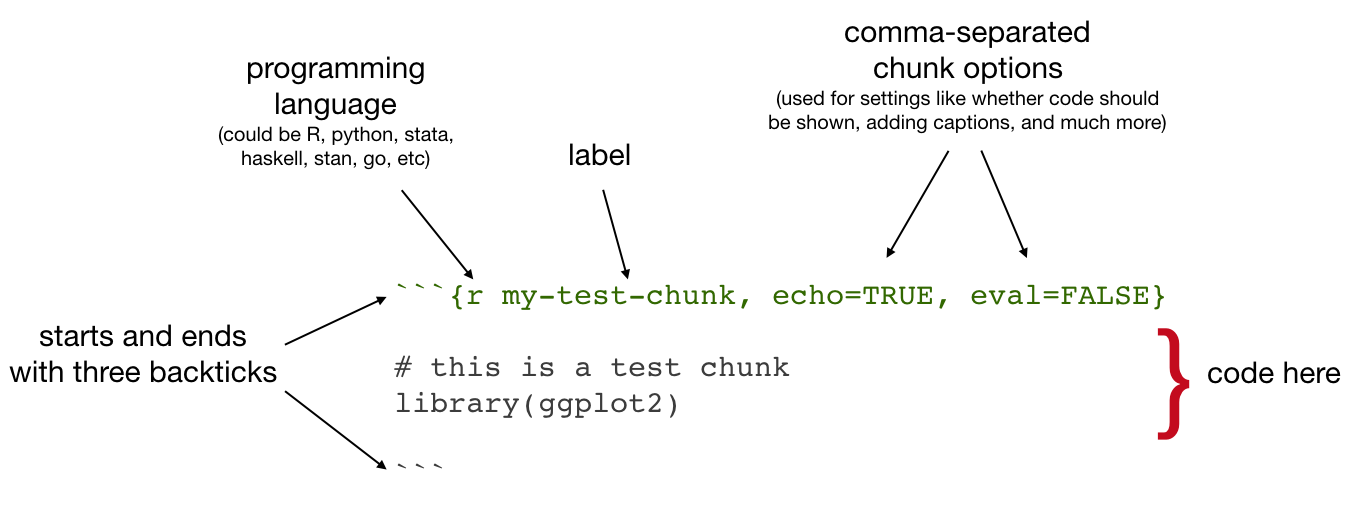
\includegraphics[width=1\linewidth]{figures/chunk-parts} \caption{Code chunk syntax}\label{fig:chunk-parts}
\end{figure}

Common chunk options include (see e.g.~\href{https://bookdown.org/yihui/rmarkdown/r-code.html}{bookdown.org}):

\begin{itemize}
\tightlist
\item
  \texttt{echo}: whether or not to display code in knitted output
\item
  \texttt{eval}: whether or to to run the code in the chunk when knitting
\item
  \texttt{include}: wheter to include anything from the from a code chunk in the output document
\item
  \texttt{fig.cap}: figure caption
\item
  \texttt{fig.scap}: short figure caption, which will be used in the `List of Figures' in the PDF front matter
\end{itemize}

\textbf{IMPORTANT}: Do \emph{not} use underscoores in your chunk labels - if you do, you are likely to get an error in PDF output saying something like ``! Package caption Error: \textbackslash caption outside float''.

\hypertarget{cross-referencing}{%
\section{Cross-referencing}\label{cross-referencing}}

We can make cross-references to \textbf{sections} within our document, as well as to \textbf{figures} (images and plots) and \textbf{tables}.

\startappendices

\hypertarget{the-first-appendix}{%
\chapter{The First Appendix}\label{the-first-appendix}}

This first appendix includes an R chunk that was hidden in the document (using \texttt{echo\ =\ FALSE}) to help with readibility:

\textbf{In 02-rmd-basics-code.Rmd}

\begin{Shaded}
\begin{Highlighting}[]
\KeywordTok{library}\NormalTok{(tidyverse)}
\NormalTok{knitr}\OperatorTok{::}\KeywordTok{include\_graphics}\NormalTok{(}\StringTok{"figures/chunk{-}parts.png"}\NormalTok{)}
\end{Highlighting}
\end{Shaded}

\textbf{And here's another one from the same chapter, i.e.~Chapter \ref{code}:}

\hypertarget{the-second-appendix-for-fun}{%
\chapter{The Second Appendix, for Fun}\label{the-second-appendix-for-fun}}

\backmatter
\end{document}
